\documentclass[aspectratio=169,11pt]{beamer}

% Theme
\usetheme{Madrid}
\usecolortheme{seahorse}
\setbeamertemplate{navigation symbols}{}
\setbeamertemplate{footline}[frame number]

% Packages
\usepackage[utf8]{inputenc}
\usepackage{graphicx}
\usepackage{amsmath,amssymb}
\usepackage{tikz}
\usetikzlibrary{shapes,arrows,positioning}

% Colors
\definecolor{threatred}{RGB}{255,107,107}
\definecolor{defensegreen}{RGB}{107,203,119}
\definecolor{processblue}{RGB}{100,149,237}
\definecolor{warningyellow}{RGB}{255,193,7}

% Title
\title[Augmented Democracy]{Augmented Democracy}
\subtitle{Procedural Coherence in Algorithmically Mediated Governance}
\author{Sylvain Cormier}
\institute{Paraxiom}
\date{December 2025}

\begin{document}

%==============================================================================
\begin{frame}
\titlepage
\end{frame}

%==============================================================================
\begin{frame}{The Problem: Democracy Under Attack}

\begin{columns}
\column{0.5\textwidth}
\textbf{Traditional Voting Assumes:}
\begin{itemize}
    \item One person, one vote
    \item Voters are informed
    \item Votes are independent
    \item Results reflect genuine preference
\end{itemize}

\column{0.5\textwidth}
\textbf{Reality in 2024:}
\begin{itemize}
    \item Sybil attacks (fake identities)
    \item Bribery and vote buying
    \item Coordinated manipulation
    \item Bot voting
    \item Information warfare
\end{itemize}
\end{columns}

\vspace{1em}
\centering
\textcolor{threatred}{\textbf{Question:} Can we detect manipulation \emph{without} deciding what's ``true''?}

\end{frame}

%==============================================================================
\begin{frame}{The Key Insight}

\begin{block}{We Cannot Algorithmically Determine Truth}
Any system claiming to verify ``facts'' must answer: \emph{who decides what counts as verified?}
\end{block}

\vspace{1em}

\begin{block}{But We Can Measure Process Quality}
Statistical properties of \emph{how} a decision was made reveal manipulation---independent of \emph{what} was decided.
\end{block}

\vspace{1em}

\centering
\Large
\textbf{Artifacts, Not Truth}

\normalsize
Facts as verifiable artifacts with provenance---not semantic claims about reality.

\end{frame}

%==============================================================================
\begin{frame}{What is Augmented Democracy?}

\begin{definition}
\textbf{Augmented Democracy} is a governance framework where:
\begin{enumerate}
    \item Human deliberation drives decisions
    \item Algorithmic infrastructure preserves process integrity
    \item The system constrains \emph{how} decisions are made
    \item The system does \textbf{not} constrain \emph{what} is decided
\end{enumerate}
\end{definition}

\vspace{1em}

\textbf{Key Properties:}
\begin{itemize}
    \item \textbf{Procedural}, not substantive
    \item \textbf{Infrastructure}, not oracle
    \item \textbf{Coherence}, not correctness
\end{itemize}

\end{frame}

%==============================================================================
\begin{frame}{The Dual Condition}

A proposal passes if and only if \textbf{both} conditions hold:

\vspace{1em}

\begin{columns}
\column{0.45\textwidth}
\begin{block}{1. Majority Condition}
\[
W_{\text{approve}} > W_{\text{reject}}
\]
Weighted votes in favor exceed those against.
\end{block}

\column{0.45\textwidth}
\begin{block}{2. Coherence Condition}
\[
\gamma > 50
\]
Process quality score exceeds threshold.
\end{block}
\end{columns}

\vspace{1em}

\centering
\textcolor{defensegreen}{\textbf{Majority alone is not sufficient.}}

\vspace{0.5em}
Even 90\% approval can be rejected if coherence indicates manipulation.

\end{frame}

%==============================================================================
\begin{frame}{What is Coherence ($\gamma$)?}

\begin{block}{Definition}
\[
\gamma = \frac{\sigma^2_\eta}{255} \times 100
\]
Entropy-weighted variance of voting patterns, normalized to [0, 100].
\end{block}

\vspace{1em}

\textbf{What it measures:}
\begin{itemize}
    \item Statistical independence of votes
    \item Proper distribution of random entropy
    \item Absence of coordinated patterns
\end{itemize}

\vspace{1em}

\textbf{What it does NOT measure:}
\begin{itemize}
    \item Whether the proposal is ``good''
    \item Whether voters made the ``right'' choice
    \item Semantic correctness of any claim
\end{itemize}

\end{frame}

%==============================================================================
\begin{frame}{The Coherence Pipeline}

\centering
\includegraphics[width=0.9\textwidth,height=0.65\textheight,keepaspectratio]{diagrams/coherence-pipeline.pdf}

\vspace{0.5em}

\textbf{Six stages, multiple gates, single invariant.}

\end{frame}

%==============================================================================
\begin{frame}{Stage 1-2: Submission and Review}

\begin{columns}
\column{0.5\textwidth}
\textbf{Proposal Submission}
\begin{itemize}
    \item Valid credential required
    \item Security deposit posted
    \item Artifact references declared
\end{itemize}

\column{0.5\textwidth}
\textbf{Review Period}
\begin{itemize}
    \item 7-day amendment window
    \item Community discussion
    \item Artifact verification
\end{itemize}
\end{columns}

\vspace{1em}

\begin{block}{Artifact Admissibility}
Referenced ``facts'' must have:
\begin{enumerate}
    \item Cryptographic hash or DOI (content-addressable)
    \item Authentic issuance (verified source)
    \item Contextual relevance (domain match)
\end{enumerate}
\end{block}

\end{frame}

%==============================================================================
\begin{frame}{Stage 3: Engagement Verification (Test Grids)}

\begin{columns}
\column{0.55\textwidth}
\textbf{Token-Curated Test Grids}
\begin{itemize}
    \item Domain-specific question pools
    \item Maintained by staked curators
    \item Voters must pass verification
    \item 70\% threshold to vote
\end{itemize}

\vspace{0.5em}
\textbf{Curator Accountability}
\begin{itemize}
    \item Slashed for \textcolor{threatred}{inaccessibility}
    \item Slashed for \textcolor{threatred}{ambiguity}
    \item Slashed for \textcolor{threatred}{irrelevance}
\end{itemize}

\column{0.4\textwidth}
\begin{alertblock}{Critical Limitation}
Curators are \textbf{never} slashed for contested conclusions.

\vspace{0.5em}
Test grids define \emph{admissibility criteria}, not semantic truth.
\end{alertblock}
\end{columns}

\end{frame}

%==============================================================================
\begin{frame}{Stage 4-5: Weighted Voting}

\textbf{Vote Weight Calculation:}
\[
w = r \times (1 + \epsilon)
\]

\begin{itemize}
    \item $r \in [0,1]$: Credential score (reputation)
    \item $\epsilon \sim \text{Uniform}(-0.1, 0.1)$: Quantum entropy injection
\end{itemize}

\vspace{1em}

\begin{columns}
\column{0.5\textwidth}
\textbf{Quadratic Voting Costs}
\[
\text{cost}(n) = n^2
\]
\begin{itemize}
    \item 1 vote costs 1 token
    \item 10 votes cost 100 tokens
    \item Reduces whale dominance
\end{itemize}

\column{0.5\textwidth}
\textbf{Life-Sustaining Credentials}
\begin{itemize}
    \item 5\% decay per epoch
    \item Participation earns bonus
    \item Inactivity accelerates decay
    \item Cannot be ``parked''
\end{itemize}
\end{columns}

\end{frame}

%==============================================================================
\begin{frame}{Stage 6: Result Determination}

\centering
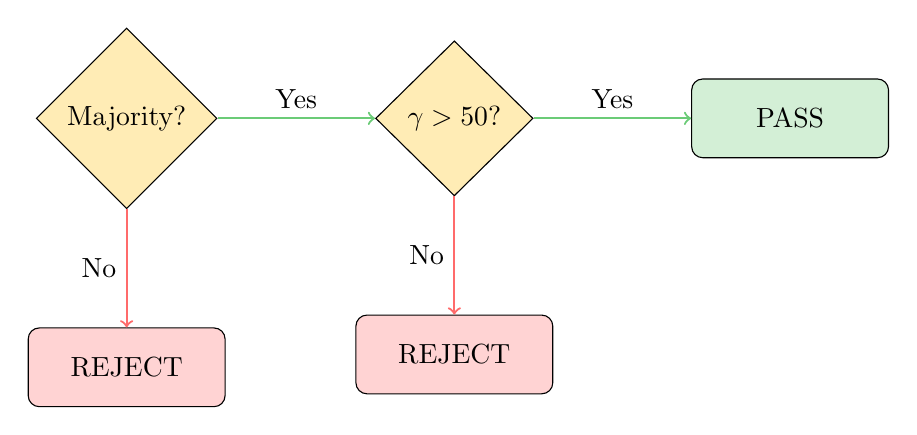
\begin{tikzpicture}[
    node distance=2cm,
    decision/.style={diamond, draw, fill=warningyellow!30, minimum width=2cm, minimum height=1cm},
    block/.style={rectangle, draw, rounded corners, minimum width=2.5cm, minimum height=1cm},
    yes/.style={->, thick, draw=defensegreen},
    no/.style={->, thick, draw=threatred}
]

\node[decision] (majority) {Majority?};
\node[decision, right=of majority] (coherence) {$\gamma > 50$?};
\node[block, fill=defensegreen!30, right=of coherence] (pass) {PASS};
\node[block, fill=threatred!30, below=1.5cm of majority] (reject1) {REJECT};
\node[block, fill=threatred!30, below=1.5cm of coherence] (reject2) {REJECT};

\draw[yes] (majority) -- node[above] {Yes} (coherence);
\draw[no] (majority) -- node[left] {No} (reject1);
\draw[yes] (coherence) -- node[above] {Yes} (pass);
\draw[no] (coherence) -- node[left] {No} (reject2);

\end{tikzpicture}

\vspace{1em}

\textbf{Both conditions must be satisfied.}

Even overwhelming majority fails without process coherence.

\end{frame}

%==============================================================================
\begin{frame}{Threat Detection Matrix}

\centering
\begin{tabular}{lcc}
\textbf{Attack Vector} & \textbf{Defense Mechanism} & \textbf{Detection Rate} \\
\hline
Sybil (fake identities) & Coherence gate ($\gamma$) & $>95\%$ for $n > \sqrt{N}$ \\
Bribery (vote buying) & Coherence + Quadratic & $>90\%$ \\
Coordinated manipulation & Coherence gate ($\gamma$) & $>95\%$ for $>10\%$ \\
Bot voting & Engagement verification & $>99\%$ \\
Unengaged voting & Test grid & $>95\%$ \\
Whale domination & Quadratic costs & Linear $\to$ Square root \\
Replay attacks & Quantum signatures & 100\% \\
\end{tabular}

\vspace{1em}

\textcolor{defensegreen}{\textbf{Key:}} Detection is statistical, not absolute. Thresholds are configurable.

\end{frame}

%==============================================================================
\begin{frame}{What Coherence Does NOT Detect}

\begin{alertblock}{Formal Limitations}
The following are \textbf{not} detected by $\gamma$:
\end{alertblock}

\begin{enumerate}
    \item \textbf{Genuine shared preferences}---Large groups with authentically similar views

    \item \textbf{Information cascades}---Organic convergence after public deliberation

    \item \textbf{Gradual ideology shift}---Slow coordination over multiple epochs

    \item \textbf{Semantic manipulation}---Proposals that are procedurally correct but substantively harmful
\end{enumerate}

\vspace{1em}

\textcolor{processblue}{\textbf{These require:}} Diverse curation, deliberation periods, human oversight, constitutional constraints.

\end{frame}

%==============================================================================
\begin{frame}{Governance as Control System}

\centering
\includegraphics[width=0.85\textwidth,height=0.6\textheight,keepaspectratio]{diagrams/control-loop.pdf}

\vspace{0.5em}

\textbf{Coherence as Lyapunov Function:} System stability proven via process quality bounds.

\end{frame}

%==============================================================================
\begin{frame}{Control-Theoretic Properties}

\begin{columns}
\column{0.5\textwidth}
\textbf{System Tuple:}
\begin{itemize}
    \item $S$: State space (parameters, treasury)
    \item $A$: Actions (proposals, votes)
    \item $T$: Transition function
    \item $I$: Invariant (dual condition)
    \item $R$: Reference (policy objectives)
\end{itemize}

\column{0.5\textwidth}
\textbf{Stability Guarantee:}
\[
\frac{d\gamma}{dt} < 0 \implies \text{instability}
\]
Declining coherence signals system degradation \emph{before} catastrophic failure.
\end{columns}

\vspace{1em}

\begin{block}{Key Property}
The system is \textbf{self-correcting}: low coherence blocks state transitions, forcing process improvement before governance can proceed.
\end{block}

\end{frame}

%==============================================================================
\begin{frame}{Historical Context}

\begin{columns}
\column{0.5\textwidth}
\textbf{Direct Democracy 1.0}
\begin{itemize}
    \item Athens, 500 BCE
    \item Physical presence
    \item Lottery selection
    \item No scalability
\end{itemize}

\vspace{0.5em}
\textbf{Representative Democracy}
\begin{itemize}
    \item 18th century onward
    \item Delegation to representatives
    \item Periodic elections
    \item Principal-agent problems
\end{itemize}

\column{0.5\textwidth}
\textbf{Liquid Democracy}
\begin{itemize}
    \item 2000s concept
    \item Transitive delegation
    \item Vote on anything
    \item Attack surface expansion
\end{itemize}

\vspace{0.5em}
\textbf{Augmented Democracy}
\begin{itemize}
    \item 2020s emergence
    \item Procedural coherence
    \item Adversarial resistance
    \item Infrastructure, not oracle
\end{itemize}
\end{columns}

\end{frame}

%==============================================================================
\begin{frame}{Failure Modes and Mitigations}

\begin{columns}
\column{0.5\textwidth}
\textbf{Technical Failures}
\begin{itemize}
    \item Entropy source compromise
    \item Oracle manipulation
    \item Smart contract bugs
\end{itemize}

\textbf{Mitigations:}
\begin{itemize}
    \item Multiple entropy sources
    \item Decentralized oracles
    \item Formal verification
\end{itemize}

\column{0.5\textwidth}
\textbf{Social Failures}
\begin{itemize}
    \item Curator capture
    \item Credential concentration
    \item Apathy decay spiral
\end{itemize}

\textbf{Mitigations:}
\begin{itemize}
    \item Curator rotation
    \item Credential caps
    \item Participation incentives
\end{itemize}
\end{columns}

\end{frame}

%==============================================================================
\begin{frame}{Implementation Status}

\textbf{Reference Implementation:}
\begin{itemize}
    \item Substrate-based runtime (Rust)
    \item EVM compatibility layer (Solidity)
    \item Quantum entropy integration
    \item IPFS artifact storage
\end{itemize}

\vspace{1em}

\textbf{Deployment Targets:}
\begin{itemize}
    \item DAO governance frameworks
    \item Municipal decision-making pilots
    \item Corporate stakeholder voting
    \item Academic institution governance
\end{itemize}

\vspace{1em}

\textbf{Open Source:} \url{github.com/paraxiom/augmented-democracy}

\end{frame}

%==============================================================================
\begin{frame}{The Scope Claim}

\begin{block}{What We Claim}
Democratic legitimacy is a \textbf{measurable property of process quality}, independent of specific outcomes.
\end{block}

\vspace{1em}

\begin{alertblock}{What We Do Not Claim}
\begin{itemize}
    \item That coherent processes produce ``correct'' outcomes
    \item That the system can determine truth
    \item That algorithms should replace human judgment
    \item That this solves all governance problems
\end{itemize}
\end{alertblock}

\vspace{1em}

\centering
\textbf{Infrastructure enables legitimate disagreement.}

\end{frame}

%==============================================================================
\begin{frame}{Conclusion: Democracy as Infrastructure}

\begin{block}{Core Thesis}
The fundamental challenge of democratic governance is \textbf{procedural integrity under adversarial conditions}---and this challenge admits algorithmic solutions that do not require resolving contested questions of truth.
\end{block}

\vspace{1em}

\textbf{Key Takeaways:}
\begin{enumerate}
    \item Process quality is measurable without semantic authority
    \item Coherence gates complement majority voting
    \item Test grids verify engagement, not correctness
    \item The system constrains process, not outcomes
\end{enumerate}

\vspace{1em}

\centering
\Large
\textbf{Questions?}

\normalsize
\texttt{sylvain@paraxiom.io}

\end{frame}

%==============================================================================
\begin{frame}[plain]
\centering
\vfill
{\Huge Thank You}

\vspace{2em}

{\large Augmented Democracy: Procedural Coherence in Algorithmically Mediated Governance}

\vspace{1em}

Paper: \texttt{paper-core.pdf}\\
Appendices: \texttt{paper-appendix.pdf}\\
Code: \url{github.com/paraxiom/augmented-democracy}

\vfill
\end{frame}

\end{document}
